En este capítulo se realizan capturas de tráfico para los comandos básicos de SNMP. Tanto las capturas como el análisis se realiza utilizando la herramienta Wireshark en Linux.
\section{Análisis de tráfico con Wireshark}
\subsection{snmpget}

En la figura \ref{image:snmpget1} podemos observar la ejecución del comando \textbf{snmpget} consultando al objeto \textbf{system}.

\FloatBarrier
\begin{figure}[htbp!]
		\centering
			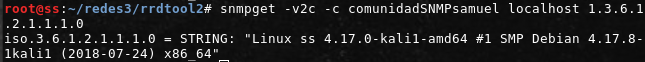
\includegraphics[width=.9 \textwidth]{images/snmpget1}
		\caption{Comando snmpget.}
		\label{image:snmpget1}
\end{figure}
\FloatBarrier

Con ello, se capturan dos paquetes: uno de solicitud y otro de respuesta mostrados en la figura \ref{image:snmpget2}.

\FloatBarrier
\begin{figure}[htbp!]
		\centering
			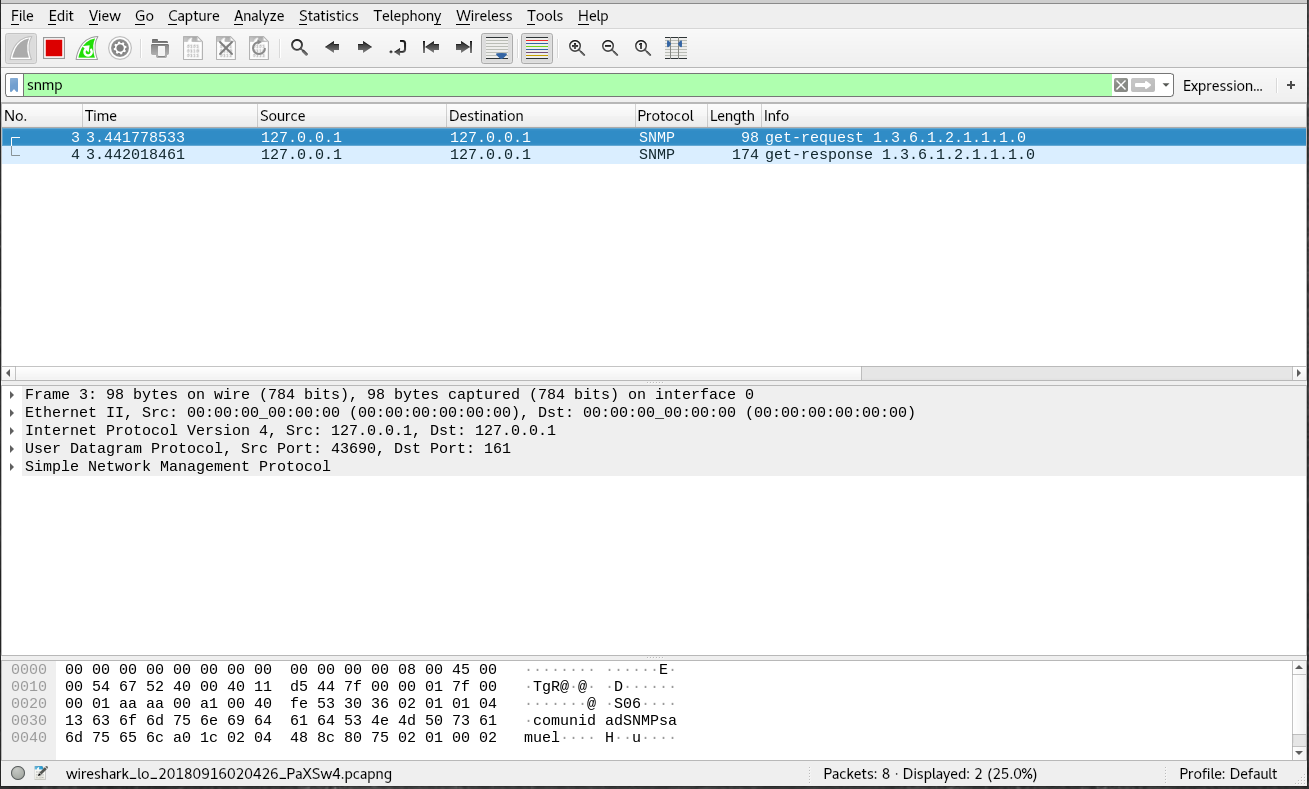
\includegraphics[width=.9 \textwidth]{images/snmpget2}
		\caption{Captura snmpget.}
		\label{image:snmpget2}
\end{figure}
\FloatBarrier

Finalmente, en las figuras \ref{image:snmpget3} y \ref{image:snmpget4} vemos la estructura de los paquetes de solicitud y respuesta respectivamente. Cabe comentar que la información transmitida con la ejecución del comando \textbf{snmpget} viaja en claro, es decir, no está cifrada.

Por un lado, observamos que en la solicitud se envía el OID, mientras que en la respuesta se envía como valor la cadena que corresponde al objeto solicitado.

\FloatBarrier
\begin{figure}[htbp!]
		\centering
			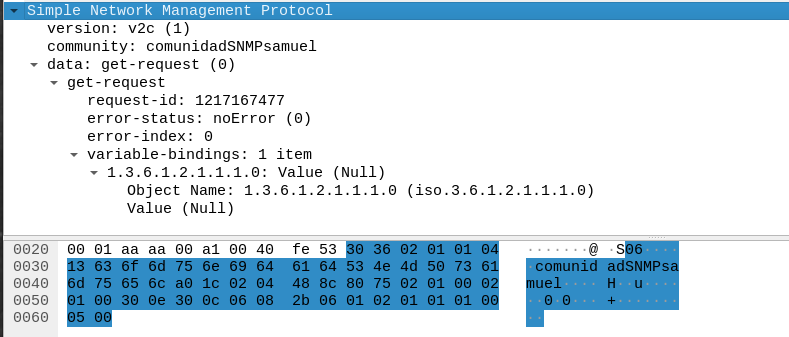
\includegraphics[width=.9 \textwidth]{images/snmpget3}
		\caption{Solicitud snmpget.}
		\label{image:snmpget3}
\end{figure}
\FloatBarrier

\FloatBarrier
\begin{figure}[htbp!]
		\centering
			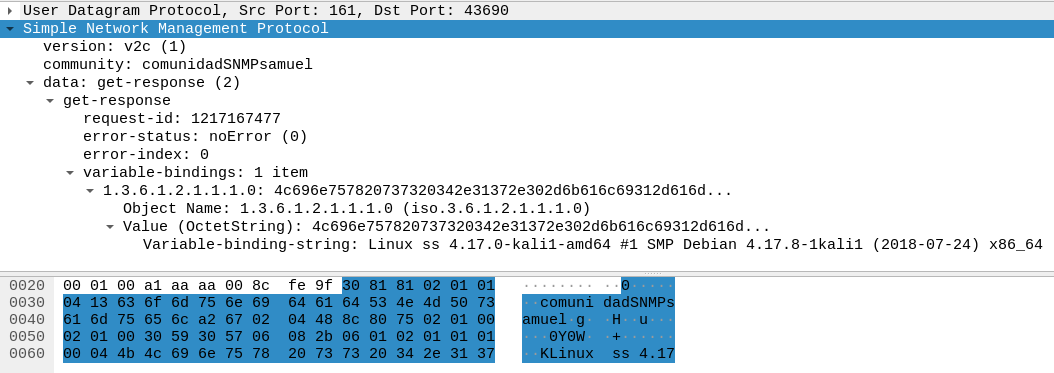
\includegraphics[width=.9 \textwidth]{images/snmpget4}
		\caption{Respuesta snmpget.}
		\label{image:snmpget4}
\end{figure}
\FloatBarrier

\subsection{snmpgetnext}

En el caso del comando \textbf{snmpgetnext}, podemos observar en la figura \ref{image:snmpgetnext1}, que se realizó la solicitud del objeto \textbf{sysUpTime} con OID 1.3.6.1.2.1.1.3.0. No obstante, el funcionamiento de \textbf{snmpgetnext} consiste en regresar el objeto siguiente. En este caso, devuelve el OID 1.3.6.1.2.1.1.4.0 \textbf{sysContact}.

\FloatBarrier
\begin{figure}[htbp!]
		\centering
			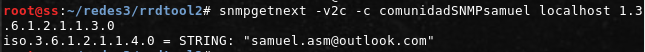
\includegraphics[width=.9 \textwidth]{images/snmpgetnext1}
		\caption{Comando snmpgetnext.}
		\label{image:snmpgetnext1}
\end{figure}
\FloatBarrier

Al observar la captura de paquetes en la figura \ref{image:snmpgetnext2}, vemos que aunque el comando ejecutado es \textbf{snmpgetnext}, se realizan peticiones y respuestas de tipo \textbf{snmpget}.

\FloatBarrier
\begin{figure}[htbp!]
		\centering
			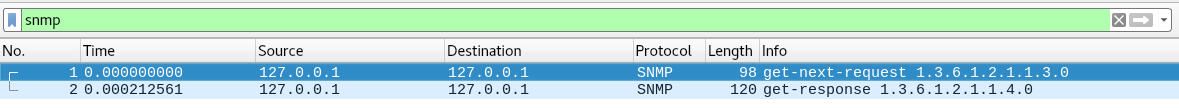
\includegraphics[width=.9 \textwidth]{images/snmpgetnext2}
		\caption{Captura snmpgetnext.}
		\label{image:snmpgetnext2}
\end{figure}
\FloatBarrier

Finalmente, en las figuras \ref{image:snmpgetnext3} y \ref{image:snmpgetnext4} vemos que los detalles de los paquetes transmitidos son de solicitud (\textbf{get-next-request}) y respuesta (\textbf{get-response}). 

\FloatBarrier
\begin{figure}[htbp!]
		\centering
			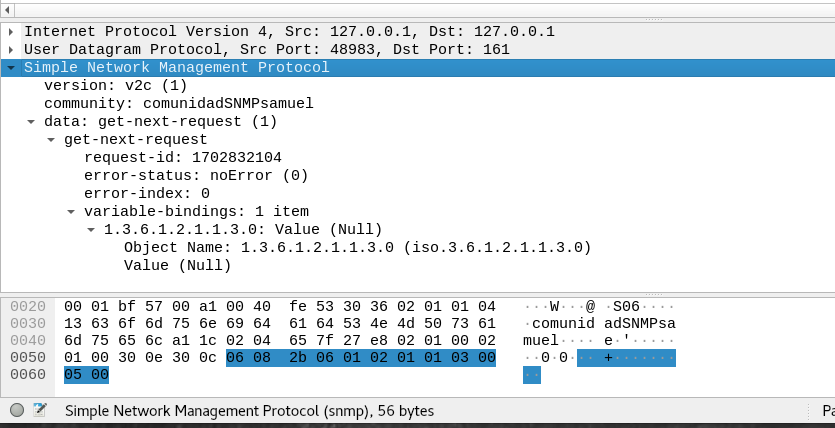
\includegraphics[width=.9 \textwidth]{images/snmpgetnext3}
		\caption{Solicitud snmpgetnext.}
		\label{image:snmpgetnext3}
\end{figure}
\FloatBarrier

\FloatBarrier
\begin{figure}[htbp!]
		\centering
			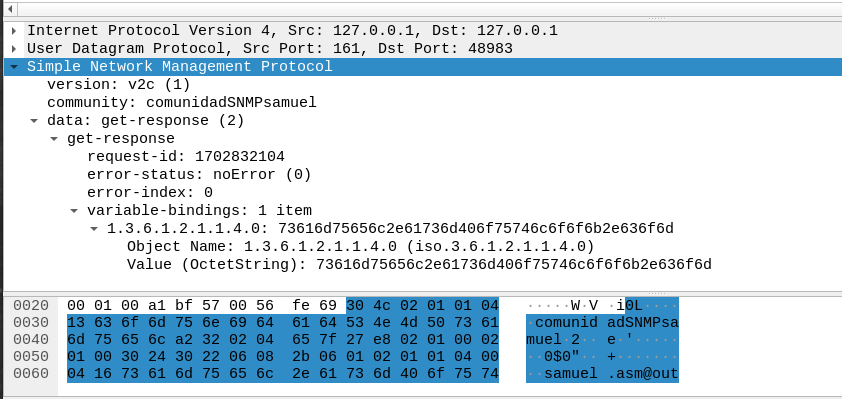
\includegraphics[width=.9 \textwidth]{images/snmpgetnext4}
		\caption{Respuesta snmpgetnext.}
		\label{image:snmpgetnext4}
\end{figure}
\FloatBarrier

\subsection{snmpwalk}

El comando \textbf{snmpwalk} realiza una serie de peticiones \textbf{snmpgetnext} automáticamente y se detiene cuando devuelve resultados que no están más dentro del rango del OID que se ingresó originalmente.

Como se muestra en la figura \ref{image:snmpwalk1}, observamos que se realizó la solicitud del OID 1.3.6.1.2.1.1. Con lo cual, se obtuvieron todos los OIDs sucesivos.

\FloatBarrier
\begin{figure}[htbp!]
		\centering
			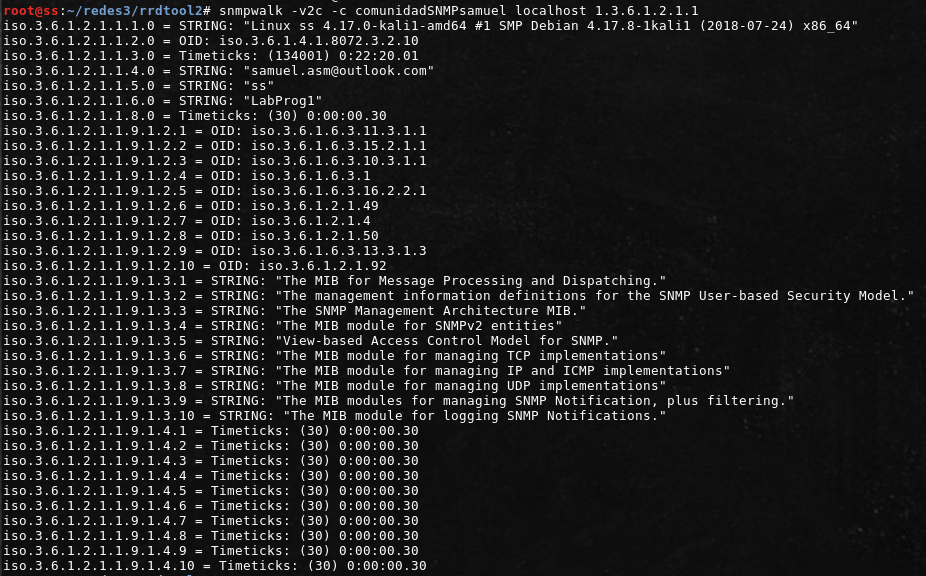
\includegraphics[width=.9 \textwidth]{images/snmpwalk1}
		\caption{Comando snmpwalk.}
		\label{image:snmpwalk1}
\end{figure}
\FloatBarrier

Respecto a los paquetes transmitidos, podemos ver en la figura \ref{image:snmpwalk2} que consisten en una serie de solicitudes (\textbf{get-next-request}) y respuestas (\textbf{get-response}).

\FloatBarrier
\begin{figure}[htbp!]
		\centering
			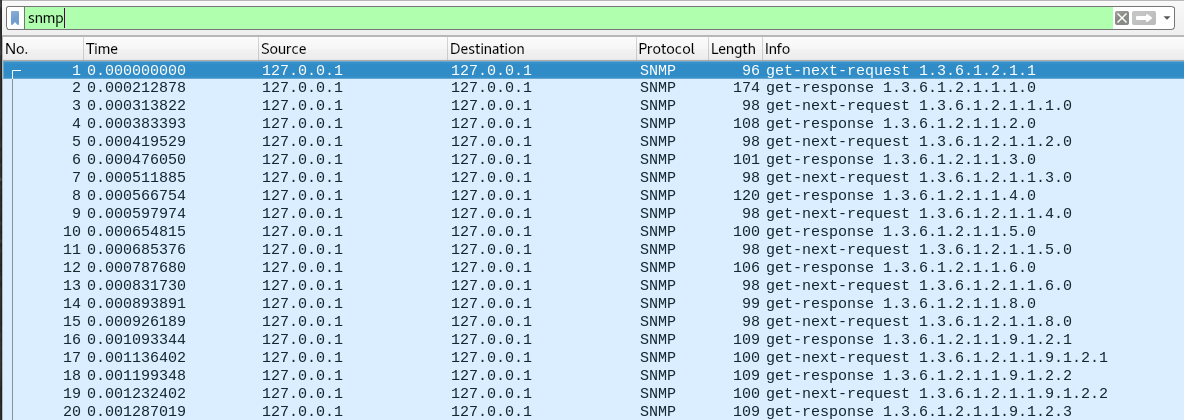
\includegraphics[width=.9 \textwidth]{images/snmpwalk2}
		\caption{Capturas snmpwalk.}
		\label{image:snmpwalk2}
\end{figure}
\FloatBarrier

\subsection{snmpset}

Como lo muestra la figura \ref{image:snmpset1}, se realizó la modificación del objeto sysContact. A pesar, de que en este caso se obtuvo un error. Podemos analizar el tráfico red generado en la figura \ref{image:snmpset2} y consiguientes.

\FloatBarrier
\begin{figure}[htbp!]
		\centering
			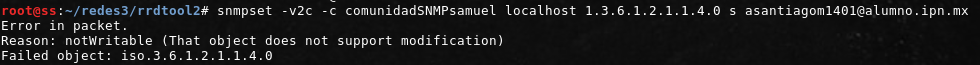
\includegraphics[width=.9 \textwidth]{images/snmpset1}
		\caption{Comando snmpset.}
		\label{image:snmpset1}
\end{figure}
\FloatBarrier

Vemos que se realiza un petición de tipo \textbf{set-request} y se obtiene una respuesta de tipo \textbf{get-response}.

\FloatBarrier
\begin{figure}[htbp!]
		\centering
			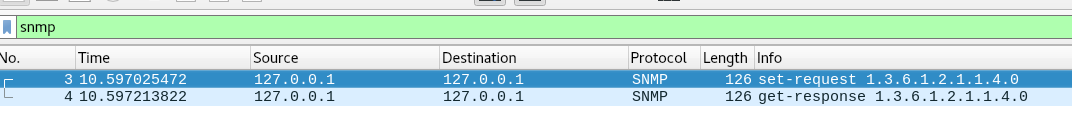
\includegraphics[width=.9 \textwidth]{images/snmpset2}
		\caption{Captura snmpset.}
		\label{image:snmpset2}
\end{figure}
\FloatBarrier

En los detalles de la solicitud de la figura \ref{image:snmpset3}, observamos que se envía un valor, el cual es la cadena que solicitamos modificar.

\FloatBarrier
\begin{figure}[htbp!]
		\centering
			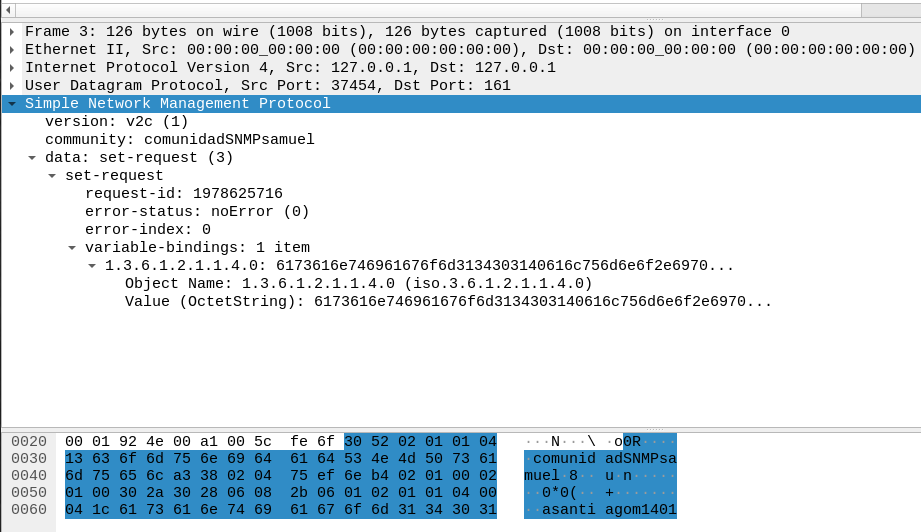
\includegraphics[width=.9 \textwidth]{images/snmpset3}
		\caption{Solicitud snmpset.}
		\label{image:snmpset3}
\end{figure}
\FloatBarrier

\FloatBarrier
\begin{figure}[htbp!]
		\centering
			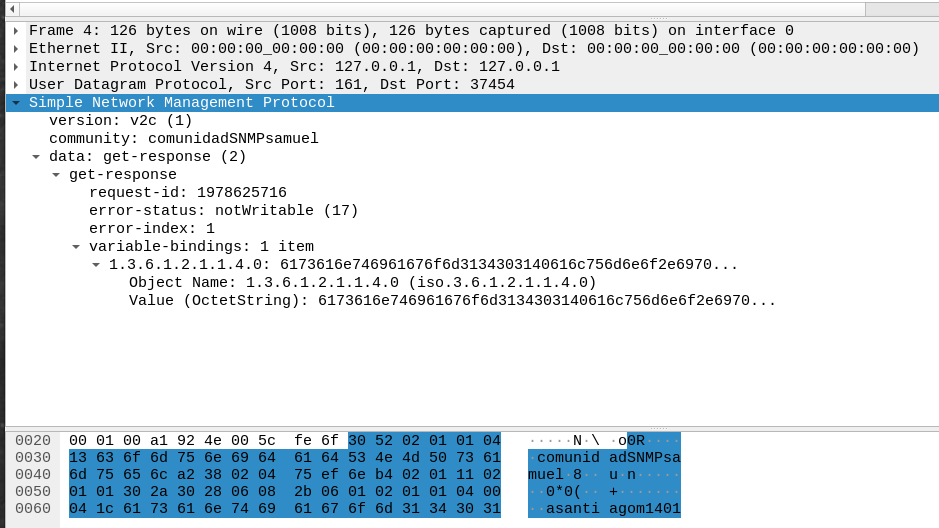
\includegraphics[width=.9 \textwidth]{images/snmpset4}
		\caption{Respuesta snmpset.}
		\label{image:snmpset4}
\end{figure}
\FloatBarrier